\section{Stacked Recommenders}
\label{sec:usermetamodeling}

\emph{Stacked Recommenders} (SR) is a way of combining recommender systems
in an effort to answer two related questions.
Given that we wish to predict the relevance of an item to a user,
using many methods that consider disjoint data patterns,

\begin{enumerate*}
  \item What rating does each method predict?
  \item How accurate will each of these predictions be?
\end{enumerate*}

User modeling methods and recommender systems traditionally only care about the first question:
a single method is used to predict an unknown rating.
Modern aggregation techniques goes one step further, and combines many methods using a generic (often weighted) combination.
However, we wish to make the aggregation \emph{adaptive},
so that the aggregation itself depends on which user and which item we are considering.

Formally, we define stacked recommenders as \emph{adapting a set of user modeling methods
with another complementary set of user modeling methods} 
(see Figure \ref{fig:stackedusermodeling}).
The first set creates standard prediction scores, and answers the first question.
The second set predicts how accurate each method will be for the current user and item,
answering the second question.
The interesting bit is that SUM can use recommender systems for both these tasks, as we shall soon see.
A system for stacked recommenders is specified by a 6-tuple:

\begin{eqnarray*}
  \mathrm{SR} &=& (Items, Users, Ratings, Framework, Methods, Adapters)\\
               &=& (I,U,R,F,M,A).
\end{eqnarray*}

\begin{figure}[t]
  \centering 
  \begin{framed}\centering
  \begin{minipage}{0.49\textwidth}
    \centering 

    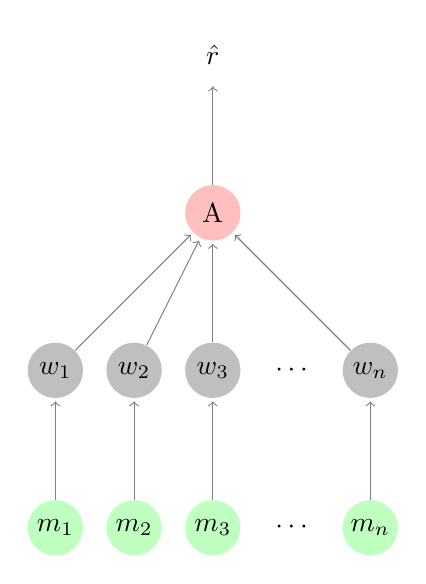
\begin{tikzpicture}[shorten >=1pt,->,draw=black!50, node distance=\layersep]
      \tikzstyle{every pin edge}=[<-,shorten <=2pt]
      \tikzstyle{node}=[circle,fill=black!25,minimum size=20pt,inner sep=0pt];
      \tikzstyle{method}=[node,fill=green!25];
      \tikzstyle{weight}=[node,fill=black!25];
      \tikzstyle{error}=[node,fill=blue!25];
      \tikzstyle{agg}=[node,fill=red!25];
      \tikzstyle{txt}=[node,fill=white];
       
      \node[method] (M1) at (0,-6) {$m_1$};      
      \node[method] (M2) at (1,-6) {$m_2$};         
      \node[method] (M3) at (2,-6) {$m_3$};         
      \node[txt]    (MS) at (3,-6) {$\cdots$}; 
      \node[method] (MN) at (4,-6) {$m_n$};
      \node[weight] (W1) at (0,-4) {$w_1$};      
      \node[weight] (W2) at (1,-4) {$w_2$};         
      \node[weight] (W3) at (2,-4) {$w_3$};         
      \node[txt]    (WS) at (3,-4) {$\cdots$}; 
      \node[weight] (WN) at (4,-4) {$w_n$};
      \node[agg]    (AG) at (2,-2) {A};
      \node[txt]    (RS) at (2,0)  {$\hat{r}$};
      
      \path (M1) edge (W1);
      \path (M2) edge (W2);
      \path (M3) edge (W3);
      \path (MN) edge (WN);
      \path (W1) edge (AG);
      \path (W2) edge (AG);
      \path (W3) edge (AG);
      \path (WN) edge (AG);
      \path (AG) edge (RS);
    \end{tikzpicture}
  \end{minipage} 
  \hfill 
  \begin{minipage}{0.49\textwidth}
    \centering 

    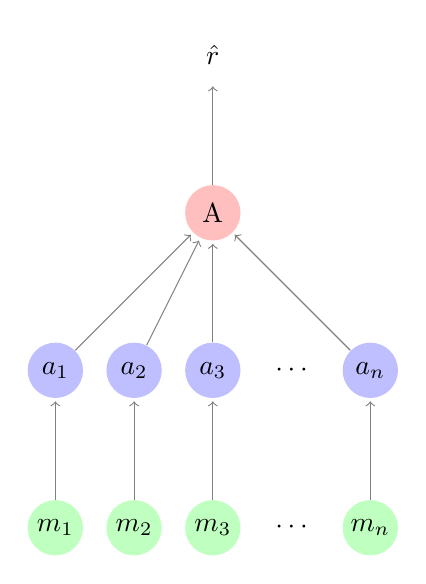
\begin{tikzpicture}[shorten >=1pt,->,draw=black!50, node distance=\layersep]
      \tikzstyle{every pin edge}=[<-,shorten <=2pt]
      \tikzstyle{node}=[circle,fill=black!25,minimum size=20pt,inner sep=0pt];
      \tikzstyle{method}=[node,fill=green!25];
      \tikzstyle{weight}=[node,fill=black!25];
      \tikzstyle{error}=[node,fill=blue!25];
      \tikzstyle{agg}=[node,fill=red!25];
      \tikzstyle{txt}=[node,fill=white];
       
      \node[method] (M1) at (0,-6) {$m_1$};      
      \node[method] (M2) at (1,-6) {$m_2$};         
      \node[method] (M3) at (2,-6) {$m_3$};         
      \node[txt]    (MS) at (3,-6) {$\cdots$}; 
      \node[method] (MN) at (4,-6) {$m_n$};
      \node[error]  (E1) at (0,-4) {$a_1$};      
      \node[error]  (E2) at (1,-4) {$a_2$};         
      \node[error]  (E3) at (2,-4) {$a_3$};         
      \node[txt]    (ES) at (3,-4) {$\cdots$}; 
      \node[error]  (EN) at (4,-4) {$a_n$};
      \node[agg]    (AG) at (2,-2) {A};
      \node[txt]    (RS) at (2,0)  {$\hat{r}$};
      
      \path (M1) edge (E1);
      \path (M2) edge (E2);
      \path (M3) edge (E3);
      \path (MN) edge (EN);
      \path (E1) edge (AG);
      \path (E2) edge (AG);
      \path (E3) edge (AG);
      \path (EN) edge (AG);
      \path (AG) edge (RS);
    \end{tikzpicture}
  \end{minipage} 
  \vspace{2em}
  \caption[Comparison of Aggregation and Adaption]{
    Comparison of aggregation and adaption:
    (left) modern aggregation approaches uses a set of pretrained weights
    to prioritize each modeling method.
    The weighted predictions are aggregated into a final prediction $\hat{r}$.
    (right) Stacked user modeling employs secondary modeling methods instead
    of weights. These estimate the accuracy of the initial method
    for the current user and item.
  }
  \label{fig:stack:comparison}
\end{framed}
\end{figure}




As always, we have sets of $Users$ and $Items$, 
and a set of $Ratings$: each user $u \in U$ can produce a rating $r \in R$ of an item $i \in I$.
Items can be just about anything: documents, websites, movies, events, or indeed, other users.
The ratings can be explicitly provided by users, for example by rating movies,
or they can be mined from existing data, for example by mining query logs.
As before, we use the term "rating" loosely --- equivalent terms include \emph{relevance}, \emph{utility},
\emph{score} or \emph{connection strength}. In other words, this is a measure of what a user thinks of an item
in the current domain language. However, since \emph{rating} will match the case study we present in the next chapter,
that is what we shall use. 

The $Framework$ variable specifies how the data is represented.
The two canonical ways of representing users, items and ratings are graphs and matrices (see Section \ref{sec:recommender}).
We shall use a matrix, where the first dimension corresponds to users, the second to items, and each populated cell is an explicit rating:

\begin{equation*}
 R_{u,i} =
 \begin{pmatrix}
  r_{1,1} & r_{1,2} & \cdots & r_{1,i} \\
  r_{2,1} & r_{2,2} & \cdots & r_{2,i} \\
  \vdots  & \vdots  & \ddots & \vdots  \\
  r_{u,1} & r_{u,2} & \cdots & r_{u,i}
 \end{pmatrix}.
\end{equation*}

As we wish to leverage disjoint data patterns, we have a set of modeling $Methods$, 
each with their own way of estimating unknown ratings. 
Each model $m \in M$ is used to compute independent and hopefully complimentary predictions.
In our case, these methods are recommendation systems.

As demonstrated in Chapter \ref{chap:theory}, there are many different recommendation algorithms,
that consider differents aspects in the data: users, items and ratings, as well as 
sources such as intra-user connections in social networks or intra-item connections in information retrieval systems.
Examples of such recommender systems include Slope One predictions, SVD factorization and Nearest Neighbor weighted predictions
(see Section \ref{subsec:recommender:examples}).
These methods predict unkown connections between users and items based on some pattern in the data,
for example user profile similarity, rating correlations or social connections.
As previously explained, to achieve the best possible combined result, we wish to use methods that look at disjoint patterns, 
i.e. complementary predictive parts of the data (see Section \ref{sec:aggregate}).

The $Adapters$ part of our 6-tuple refers to the second level of user modeling methods.
In traditional prediction aggregation this is a simple linear function for combining the different predictions,
for example by precomputing a set of weights, one for each method.
As found by \citet[p6]{Bell2007} the accuracy of the combined predictor is more dependent on the 
ability of the various predictors to expose different aspects of the data, than on 
the individual accuracy of each predictor.
As described in Section \ref{sec:aggregate}, multiple prediction results are normally 
combined into a final singular result,
based on a generalized combination found by minimizing some error across all users.

With stacked recommenders, the $Adapters$ are themselves user modeling methods 
(see Figure \ref{fig:stack:comparison}).
Methods in this second layer are used to predict how accurate each of their corresponding basic recommenders will be.
It is these methods that will allow us to do adaptive aggregation based on the current user and item.
In other words, we have two distinct layers of user modeling 
(see Figure \ref{fig:stackedusermodeling}):

\begin{figure}[t]
  \center
  \def\layersep{2cm}
  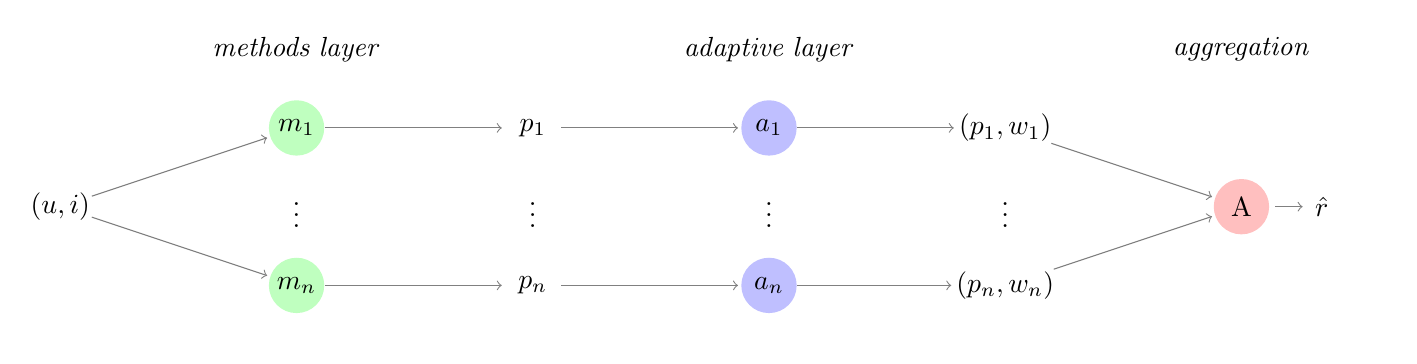
\begin{tikzpicture}[shorten >=1pt,->,draw=black!50, node distance=\layersep]

    \tikzstyle{every pin edge}=[<-,shorten <=2pt]
    \tikzstyle{node}=[circle,fill=black!25,minimum size=20pt,inner sep=0pt]
    \tikzstyle{input node}=[node, fill=green!25];
    \tikzstyle{output node}=[node, fill=red!25];
    \tikzstyle{hidden node}=[node, fill=blue!25];
    \tikzstyle{annot} = [text width=10em, text centered]
    \tikzstyle{txt}=[node,fill=white];
    
    \node[txt] (UI) at (0,-2) {$(u,i)$};  

    \node[input node] (I-1) at (\layersep,-1) {$m_1$};
    \node[txt]        (I-D) at (\layersep,-2) {$\vdots$};
    \node[input node] (I-N) at (\layersep,-3) {$m_n$};
    
    \node[txt] (P-1) at (\layersep*2, -1) {$p_1$};
    \node[txt] (P-D) at (\layersep*2, -2) {$\vdots$};
    \node[txt] (P-N) at (\layersep*2, -3) {$p_n$};

    \node[hidden node] (H-1) at (\layersep*3, -1) {$a_1$};    
    \node[txt]         (H-D) at (\layersep*3, -2) {$\vdots$};    
    \node[hidden node] (H-N) at (\layersep*3, -3) {$a_n$};    

    \node[txt] (R-1) at (\layersep*4, -1) {$(p_1,w_1)$};
    \node[txt] (R-D) at (\layersep*4, -2) {$\vdots$};
    \node[txt] (R-N) at (\layersep*4, -3) {$(p_n,w_n)$};
    
    % hidden helper node
    \node[txt] (HH)  at (\layersep*5,-1) {};

    % Draw the output layer node
    \node[output node,pin={[pin edge={->}]right:$\hat{r}$}] at (\layersep*5,-2) (O) {A};
    
    \path (UI) edge (I-1);
    \path (UI) edge (I-N);

    \path (I-1) edge (P-1);
    \path (I-N) edge (P-N);

    \path (P-1) edge (H-1);
    \path (P-N) edge (H-N);

    \path (H-1) edge (R-1);
    \path (H-N) edge (R-N);

    \path (R-1) edge (O);
    \path (R-N) edge (O);

    % Annotate the layers
    \node[annot,above of=I-1, node distance=1cm] {\emph{methods layer}};
    \node[annot,above of=H-1, node distance=1cm] {\emph{adaptive layer}};
    \node[annot,above of=HH,  node distance=1cm] {\emph{aggregation}};
  \end{tikzpicture}

  \vspace{1em}
  \caption[Stacked User Modeling]{
    Stacked user modeling:
    The method layer consists of ordinary modeling methods,
    each predicting the rating between a user and an item.
    This produces a set of predicted ratings ($p$).
    The adaptive layer estimates how well each modeling method
    will perform for the current user and item,
    and weighs the predictions accordingly.
    This produces a set of predictions and weights [$(p,w)$].
    The aggregation weighs the predictions into a final score $\hat{r}$.  
  }
  \label{fig:stackedusermodeling}
\end{figure}


\begin{enumerate}
  \item
    \emph{The methods layer} consists of traditional user modeling methods, that use a single aspect of the data to produce predictions.
    When presented with an item and a user, these methods produce a predicted rating $\hat{r}_{ui}$ based on their algorithms.
  \item
    \emph{The adaptive layer} is another set of corresponding modeling methods, that work a bit differently.
    These methods take an item and a user and estimates how well its underlying method will perform this prediction.
    The accuracy estimations are then combined with the predictions by aggregation.
    Each of these adaptive methods do not have to employ the same algorithm as their corresponding methods,
    the layers are only similar in that both consist of recommender systems.
\end{enumerate}

:::::::::::::::::::::::::::::::::::::::::::::::::::::::

Another way of describing (and implementing) the two modeling levels is through application
of the $\mathrm{map}$ and $\mathrm{reduce}$ functions of functional programming.
When performing \emph{prediction aggregation} (scores), this estimation can be expressed as

\begin{equation*}
  \hat{r}_{ui} = \mathrm{reduce}(u, i, \mathrm{map}(M, u, i)).
\end{equation*}

First, each modeling method is applied through the $\mathrm{map}$ function, with the current user and item for which
a rating should be estimated. This operation returns a set of scalar prediction values. These values are then
combined in the $\mathrm{reduce}$ method, which takes the predictions and current user as input.
In our case, this is the set of adaptive recommender methods. 
If we wish to do rank aggregation (i.e. sorted lists), the equation is a bit different:

\begin{equation*}
  \tau_{u,n} = \mathrm{reduce}(u, \mathrm{map}(M,u,n)).
\end{equation*}

Here, $\tau_{u}$ is the list of recommended items for user $u$ (following the notation in \citet[p3]{Dwork2001}).
Note that there is no input item in this formula as we wish to produce a ranking of the top $n$ recommended items.

Expressing ourselves in terms of $\mathrm{map}$ and $\mathrm{reduce}$ now is helpful, as this will later
guide our implementation of these operations in a proper MapReduce framework
for parallell computation (as explained in \citet[p75]{Manning2008}).
The $\mathrm{map}$ function may apply each modeling method in parallell, 
as these are independent computations.
The modified $\mathrm{reduce}$ function, which takes the resulting predictions $\mathrm{map}$ and the current
user as inputs, serve as our adaptive layer.


\subsection{Adaptive Aggregation}

To perform adaptive aggregation, we need the $Adapters$ to be actual recommender systems.
Until now we have talked about both prediction aggregation (scores) and rank aggregation (sorted lists).
For now we shall stick to scalar predictions, but will return to rank aggregation in Section \ref{sec:methods:rank}.
The simplest generalized way of prediction aggregation is to take the avereage of all predictions made
by the different methods (e.g. \citet[p3]{Aslam2001}):

\begin{equation*}
  \hat{r}_{ui} = \frac{1}{N} \sum_{m \in M} p(m,u,i).
\end{equation*}

Here, $\hat{r}_{ui}$ is the estimated rating from user $u$ to item $i$,
$N$ is the number of methods in $M$, and $p(m,u,i)$ is the predicted rating from method $m$.
However, most recommender aggregators attempt to weigh each method differently (e.g. \cite{Claypool1999}):

\begin{equation*}
  \hat{r}_{ui} = \sum_{m \in M} w_{m} \cdot p(m,u,i) 
  \quad \text{where} \quad 0 \leq w_{m} \leq 1, \quad \sum_{i \in M} (w_i) = 1.
\end{equation*}

Here, $w_m$ is the weight applied to modeling method $m$. These weights fall in the range $[0,1]$ and sum up to $1$.
As described in \ref{sec:aggregate}, these weights can be estimated through different machine learning methods.
Most often, the ratings data is divided into two sets:
A training set for training the recommender systems, and a testing set for finding the weights
that produce the optimal combination of predictors.
However, as discussed in Section \ref{sec:reasoning},
this is still a generalized result, averaged across every user. 
The system assumes that the best average result is the best result for each individual user.

In order to leverage as many data patterns as possible, and remove the latent subjectivity,
we need \emph{adaptive weights} that are computed spcifically for each combination of a user and an item.
However, just as we do not know the rating of every combination, we do not know the optimal weight.
In other words, these adaptive weights have to be estimated, just as the ratings themselves:

\begin{equation*}
  \hat{r}_{ui} = \sum_{m \in M} p_{w}(m,u,i) \cdot p_{r}(m,u,i)
  \quad \text{where} \quad
  \sum_{m \in M} (p_{w}(m,u,i)) = 1.
\end{equation*}

We have now reduced our mission to creating a method that can estimate the adaptive weights: $p_{w}(m,u,i)$.
As mentioned, we wish to use the same algorithms for both of these predictions.
For recommender systems to be applicable here, we need to create a matrix (or graph)
that stores known estimations of how accurate some of the predictions will be.

\begin{figure}[t]
  \center
  \def\layersep{3cm}
  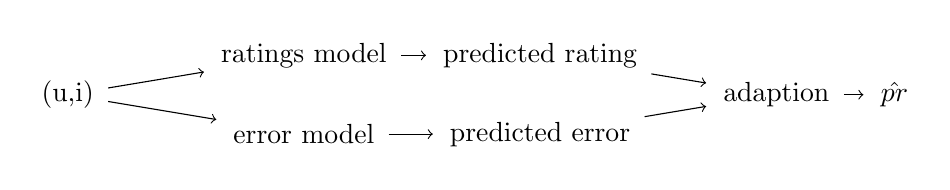
\begin{tikzpicture}[shorten >=1pt,->,draw=black, node distance=\layersep]

    \tikzstyle{every pin edge}=[<-,shorten <=2pt]
    \tikzstyle{rmodel}=[rectangle,fill=green!25,minimum size=20pt,inner sep=5pt]
    \tikzstyle{emodel}=[rectangle,fill=blue!25,minimum size=20pt,inner sep=5pt]
    \tikzstyle{amodel}=[rectangle,fill=red!25,minimum size=20pt,inner sep=5pt]
    \tikzstyle{blank}=[rectangle,fill=white,minimum size=20pt,inner sep=5pt]
    
    \node[blank] (UI) at (0,-0.5) {(u,i)}; 

    \node[blank] (EM) at (\layersep,-1) {error model};
    \node[blank] (RM) at (\layersep,0) {ratings model};
    
    \node[blank] (ER) at (\layersep*2,-1) {predicted error};
    \node[blank] (RR) at (\layersep*2,0) {predicted rating};
 
    \node[blank] (AG) at (\layersep*3,-0.5) {adaption};
    \node[blank] (W) at (\layersep*3.5,-0.5) {$\hat{pr}$}; 
    
    \path (UI) edge (EM);
    \path (UI) edge (RM);
    \path (EM) edge (ER);
    \path (RM) edge (RR);
    \path (ER) edge (AG);
    \path (RR) edge (AG);
    \path (AG) edge (W);
       
  \end{tikzpicture}

  \vspace{1em}
  \caption[Multiple Models for Adaptive Weights]{
    Multiple models for adaptive weights: 
    The data flow through the adaption of a single recommender method.
    The current user and item is fed into two distinct models: the ratings model, which 
    predicts unknown ratings, and the error model, which predicts how accurate 
    this rating will be for the current input. 
    The two predictions are then aggregated into a final part of a rating ($\hat{pr}$).
    Each of the recommender stacks contribute parts to the final rating.
  }
  \label{fig:adaptiveweights}
\end{figure}


The key insight is that \emph{the accuracy of a method is the inverse of its predicted error}.
By modeling the errors of a method through standard recommender systems,
we can in turn predict errors for untested combinations
(see Figure \ref{fig:adaptiveweights}).
Consider the following \emph{error matrix}:

\begin{equation*}
 E_{u,i} =
 \begin{pmatrix}
    e_{1,1} & e_{1,2} & \cdots & e_{1,i} \\
    e_{2,1} & e_{2,2} & \cdots & e_{2,i} \\
    \vdots  & \vdots  & \ddots & \vdots  \\
    e_{u,1} & e_{u,2} & \cdots & e_{u,i}
 \end{pmatrix}
\end{equation*}

Creating an error matrix for each modeling method is quite simple:
by splitting the ratings data in two,
the first set can be used for the actual training, and the second
can be used to populate each error matrix.
Each standard modeling method gets an error matrix where some cells have values:
each value corresponds to the prediction error for a combination of a user and an item.
Notice how similar this matrix is to the previously introduced ratings matrix.
This similarity is what will allow us using the exact same modeling methods
to perform adaptive aggregation.
Whenever we wish to train a new modeling method,
\emph{the modeling phase}, we apply the following algorithm:

\begin{enumerate*}
  \item Split the ratings data into two sets for training and error estimation.
  \item Train the modeling method in its specific way with the first training set.
  \item Use the error estimation data set to create the error matrix.
  \item Train a meta modeling method (error model) based on the error matrix.
\end{enumerate*}

When we have an error model for each modeling method, 
we can use these errors to estimate each weight.
Whenever we wish to create an adaptive aggregate prediction,
\emph{the prediction phase},
we apply the following algorithm:

\begin{enumerate*}
  \item Collect predictions from each modeling method for $(u,i)$.
  \item Collect estimated errors for each method for $(u,i)$.
  \item Normalize the errors so that the error vector sums to $1$.
  \item Compute a weighted combination where each weight is $1 - e_{m,u,i}$.
\end{enumerate*}

The next section will explain these steps in detail.
For now, we have our approach to stacking recommenders:

\begin{equation*}
  \hat{r}_{ui} = \sum_{(m_{e}, m_{r}) \in M} (1 - p(m_{e},u,i)) \cdot p(m_{r},u,i),
\end{equation*}

where $p$ returns a prediction from a model for a specific user and item,
$m_{r}$ is a standard recommender model, 
and $m_{e}$ is its corresponding error model.
For this equation to work as expected, the weights must be normalized:

\begin{equation*}
  0 \leq p_{e}(m,u,i) \leq 1 \quad \text{and} \quad \sum_{m \in M} (p_{e}(m,u,i)) = 1.
\end{equation*}

Notice that the \emph{only} difference between $m_e$ and $m_r$ is how they are created.
$m_r$ is trained with the standard ratings matrix, and $m_e$ is trained using the error matrix.
This means we can use \emph{any} standard modeling method to perform adaptive aggregation.
Hence, the name \emph{stacked recommenders}: 
each standard modeling method is stacked under another accuracy estimating modeling method.

The result of this is a system that does not only aggregate a number of predictions for each unknown
combination of users and items,
but that also combines these methods based on how accurate each prediction is likely to be.
Now that we have our model, it is time to see how it can be implemented.
First, we shall do prediction aggregation in a recommendation scenario,
and then rank aggregation in an information retrieval scenario.

\clearpage
